\begin{figure}[htbp]
	\centering
	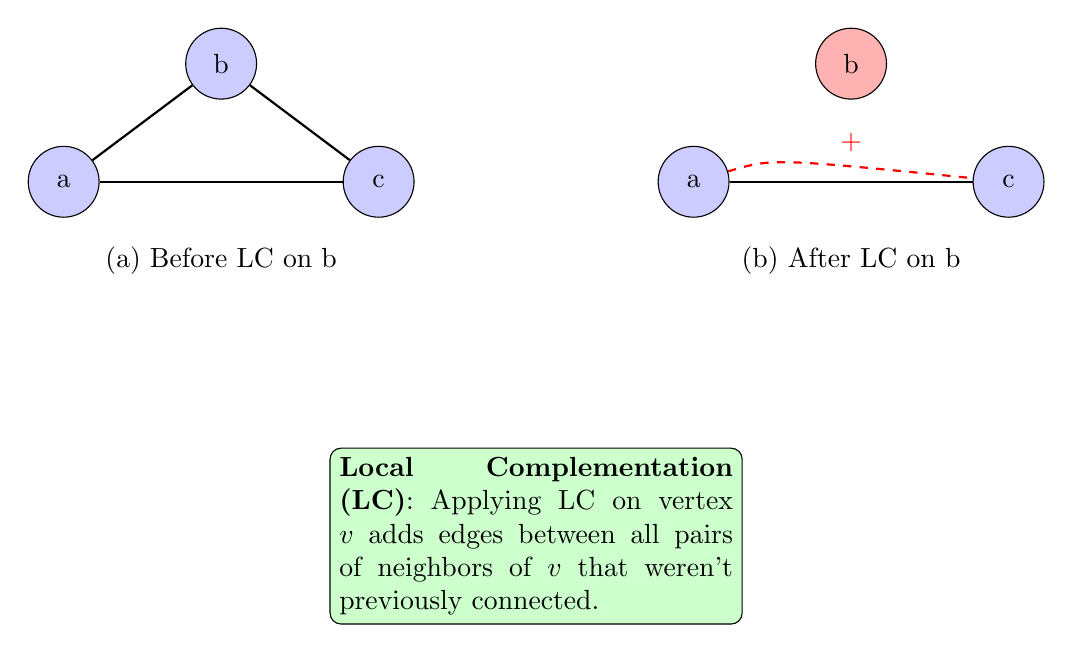
\begin{tikzpicture}
		\node[draw, circle, fill=blue!20, minimum size=0.9cm] (a) at (0,0) {a};
		\node[draw, circle, fill=blue!20, minimum size=0.9cm] (b) at (2,1.5) {b};
		\node[draw, circle, fill=blue!20, minimum size=0.9cm] (c) at (4,0) {c};

		\draw[thick] (a) -- (b);
		\draw[thick] (b) -- (c);
		\draw[thick] (a) -- (c);

		\node at (2,-1) {(a) Before LC on b};

		\node[draw, circle, fill=blue!20, minimum size=0.9cm] (a2) at (8,0) {a};
		\node[draw, circle, fill=red!30, minimum size=0.9cm] (b2) at (10,1.5) {b};
		\node[draw, circle, fill=blue!20, minimum size=0.9cm] (c2) at (12,0) {c};

		\draw[thick] (a2) -- (c2);
		\draw[dashed, red, thick] (a2) .. controls (9,0.3) .. (c2);
		\draw[red] (10,0.5) node {$+$};

		\node at (10,-1) {(b) After LC on b};

		\node[draw, rounded corners, fill=green!20] at (6,-4.5) {
			\begin{minipage}{5cm}
				\textbf{Local Complementation (LC)}: Applying LC on vertex $v$ adds edges between all pairs of neighbors of $v$ that weren't previously connected.
			\end{minipage}
		};
	\end{tikzpicture}
	\caption{Illustration of local complementation on a graph state. When LC is applied to vertex $b$, an edge is added between its neighbors $a$ and $c$. States related by LC (and edge additions/deletions) have equivalent entanglement structure.}
	\label{fig:local-complementation}
\end{figure}
